\def\difficulty{1}
\sujet{2D Fourier Transform}

\begin{note}The main objective of this tutorial is to study image filters applied in the frequencial or spatial domain with the Fourier transform. \end{note}

\begin{mcomment}
\begin{mremark}
Use  \minline{fft2}, \minline{ifft2}, \minline{fftshift} functions to compute the Fourier Transform, \minline{angle} and \minline{abs} for phase and amplitude.
\end{mremark}
\end{mcomment}
\begin{pcomment}
\begin{premark}
Use module \pinline{np.fft}  for Fourier Transform functions (function \pinline{fft2}), \pinline{phase} and \pinline{abs} for phase and amplitude.
\end{premark}
\end{pcomment}

\noindent The image to be used comes from a human cornea endothelium observed ex vivo by optical microscopy. 

\begin{figure}[htbp]
\centering\caption{Image of human cornea endothelium observed by optical microscopy. The ophthalmologists would like to know the cell density, without manually counting all the cells.}%
\subfloat[Human corneal endothelium, extracted from a donor and observed here before grafting.]{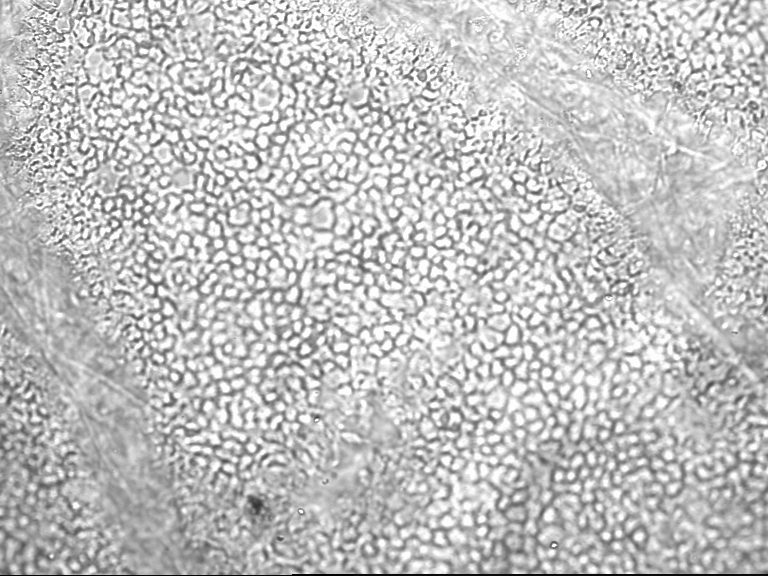
\includegraphics[width=.45\linewidth]{cornee.png}}\hfill
\subfloat[Human eye (from Wikipedia, authors: Rhcastilhos and Jmarchn, CC-By-SA).]{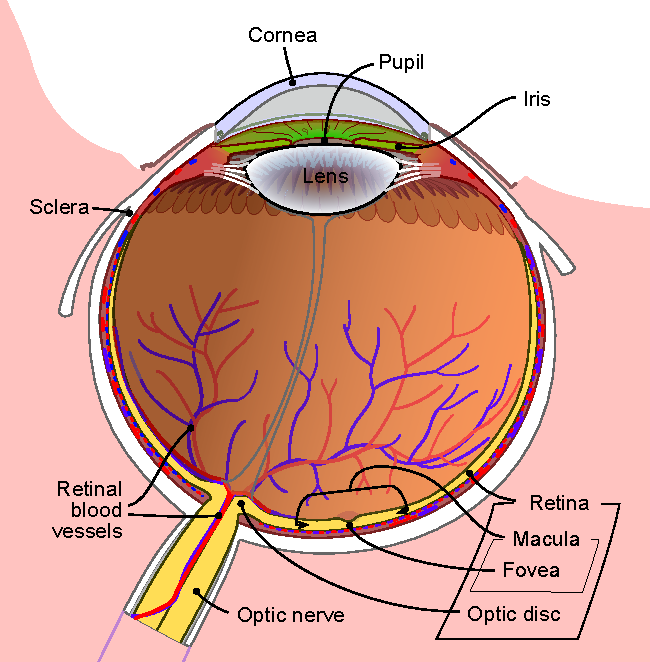
\includegraphics[width=.45\linewidth]{human_eye.pdf}}%
\label{fig:cornea}
\end{figure}

\section{Fourier transform}
\index{Fourier Transform!2D FFT}

\begin{qbox}
\begin{enumerate}
	\item Load an image and visualise it.
	\item Compute the Fourier Transform by the fft algorithm.
	\item Visualise the images of the phase and amplitude of the Fourier Transform.
\end{enumerate}
\end{qbox}

\section{Inverse Fourier transform}
\index{Fourier Transform!Inverse}
In this exercise, it can be interesting to consider different images, like a Lena picture for example.

\begin{qbox}
\begin{enumerate}
 \item Apply the inverse Fourier transform on the Fourier transform to find the original image.
 \item Now, apply the inverse Fourier transform on the phase information only (without using the frequency informations).
 \item In a same spirit, apply the inverse Fourier transform on the frequency informations only (without the phase).
\end{enumerate}
\end{qbox}

\section{Low-pass and high-pass filtering}\index{Fourier Transform!Filtering}
\begin{qbox}
\begin{enumerate}
	\item Modify the Fourier transform of the image to 
	\begin{itemize}\item keep only low frequencies,
	 \item keep only high frequencies.
	\end{itemize}
 
	\item Apply the inverse Fourier transform on both and comment. 
\end{enumerate}
\end{qbox}


%%%%%%%%%%%%%%%%%%%%%%%%%%%%%%%%%%%%%%%%%%%%%%%%%%%%%%%%%
\section{Application: evaluation of cellular density}\index{Fourier Transform!Application}
The ophthalmologists would like to evaluate the cell density of the cornea endothelium observed in Fig. \ref{fig:cornea}. %For this purpose, we consider that one cell is a pattern that is repeated at a certain frequency, that is somehow related to the cell density.

\begin{qbox}
\begin{enumerate}
\item Compute the Fourier transform of the image. If one considers that the cells constitute a repeated pattern on the whole image, locate the repetition frequency on the amplitude image.
\item Can this frequency be linked to the cell density~?
\end{enumerate}
\end{qbox}

The answer to this last question is obviously yes. Here follows a simple method to evaluate the cell density (or the mean cell radius), if these cells a considered as circular \cite{Selig2015}.

\begin{qbox}
\begin{enumerate}
 \item The amplitude information is very noisy. First of all, a gaussian filter should be applied (see functions \minline!fspecial! and \minline!imfilter!).
 \item Find a simple way to evaluate the mean radius of the cells.
\end{enumerate}
\end{qbox}

